\documentclass[ngerman,openany, oneside]{Script}
\usepackage{amsmath}


% Aufgabentext ein-/ausschalten
\newboolean{aufgabentext}
\setboolean{aufgabentext}{true}
\newcommand{\aufgabentext}[1]{\ifthenelse{\boolean{aufgabentext}}{#1}{}}

% Wenn aufgabentext auch true ist, dann wird der Lösungstext etwas abgesetzt und kursiv geschrieben
\newboolean{mitloesung}
\setboolean{mitloesung}{false}
\newcommand{\loesung}[1]{\ifthenelse{\boolean{mitloesung}}{\ifthenelse{\boolean{aufgabentext}}{{~\\\itshape{#1}}}{#1}}{}}

% Für die Strukturierung
\newcommand{\Thema}[1]{\chapter{#1}}
\newcommand{\Thementeil}[1]{\section{#1}}
\newcommand{\Aufgabe}[1]{\subsection{#1}}
\newcommand{\Unteraufgabe}[1]{\subsubsection{#1}}
\newcommand{\Lernziele}[1]{\subsection*{Lernziele}{#1}}
\graphicspath{{./Bilder/}}

\begin{document}

\titelseite[Christian Stoll\\ Sebastian Lange]{Das Praxisskript }%
	{für den Amateurfunkkurs Klasse A}%
	{SoSe 2016}%

\newpage
\thispagestyle{empty}

\begin{tabular}{p{13cm} p{1cm}}
\textbf{Impressum} &\\
&\\
Titel: Praxisskript der Projektwerkstatt DK0TU&\\
Autor: Christian Stoll&\\
1. Auflage Juni 2016 &\\
&\\
Erschienen im :&\\
Fachgebiet Hochfrequenztechnik &\\
Institut für Hochfrequenz- und Halbleiter-Systemtechnologien&\\
Fakultät IV - Elektrotechnik und Informatik &\\
Sekr. HFT 4 &\\
Raum HFT 307 &\\
Einsteinufer 25 &\\
D-10587 Berlin &\\
&\\
Leitung: Prof. Dr. Klaus Petermann &\\
&\\
&\\
%Abbildung:&\\
&\\
Aktuelle Informationen der Projektwerkstatt finden Sie unter:  &\\
\url{http://www.dk0tu.de} &\\
&\\
Die vorliegende Fassung des Praxisskripts wurde sorgfältigst auf Fehler hin überprüft. Um das Praxisskript dennoch laufend verbessern zu können, würden wir uns über Hinweise auf etwaig vorhandene Fehler sowie Verbesserungsvorschläge sehr freuen. Wenden Sie sich dazu bitte an die Tutor\_innen und wissenschaftlichen Mitarbeiter\_innen der Projektwerkstatt. &\\
\end{tabular}




\newpage
%%Inhaltsverzeichnis
\tableofcontents
\newpage

\newpage

\chapter{Die Spule}

%https://de.wikipedia.org/wiki/Datei:Electronic_component_inductors.jpg

\begin{wrapfigure}[0]{r}[-1cm]{3cm}
 \vspace{-5cm}
 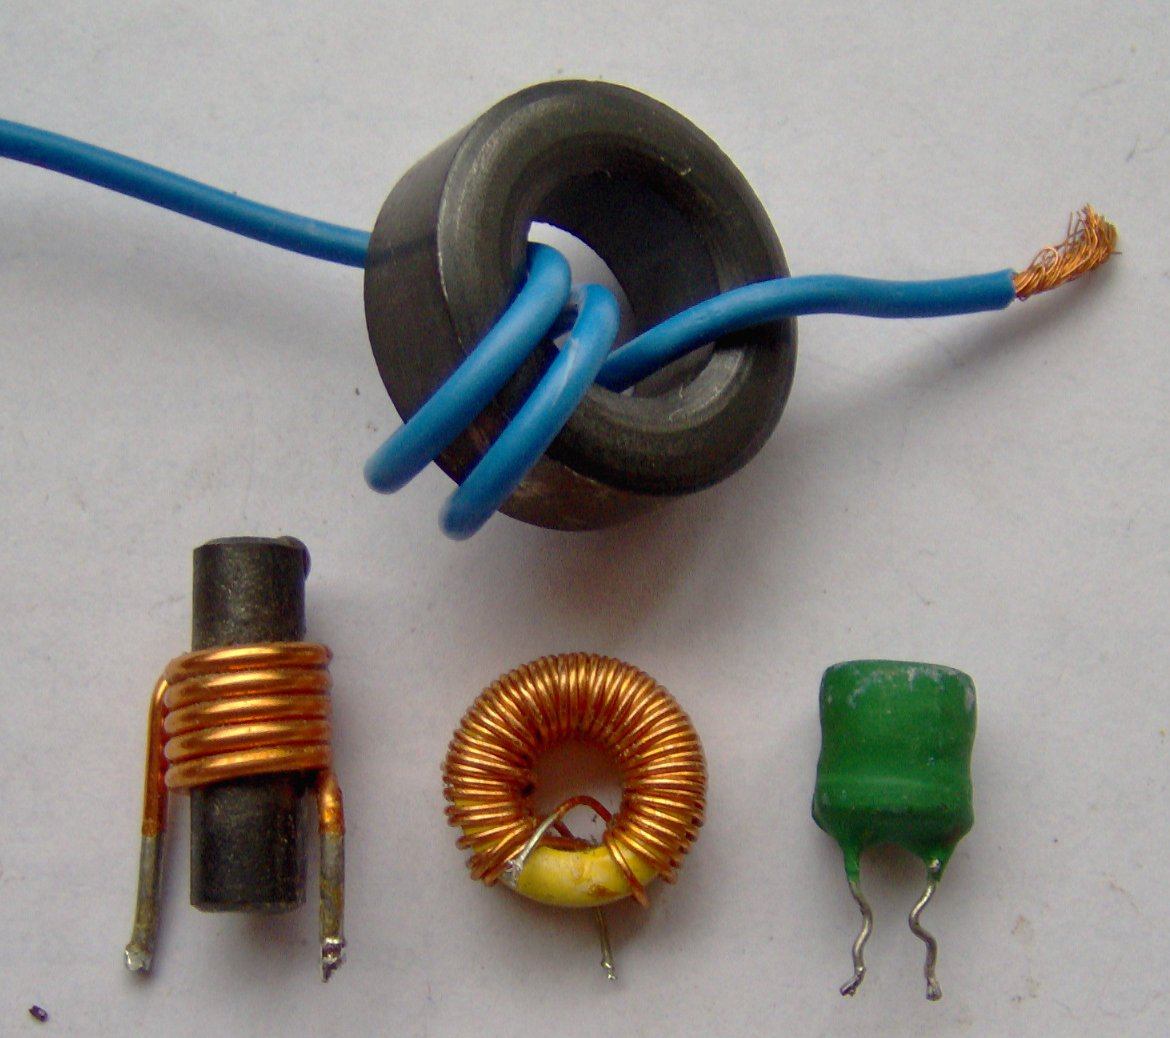
\includegraphics[scale=0.1]{Spule/Bilder/Electronic_component_inductors.jpg}
 \vspace{-5cm}
\end{wrapfigure}

\section*{Theorie- und Prüfungsfragen} 
~~~
\begin{enumerate}
\itemsep1pt\parskip0pt\parsep0pt
\item[1] Wie lässt sich die Induktivität einer Spule berechnen?
\item[2] Wie lautet die magnetische Feldkonstante $\mu_0$?
\item[3] Wie lautet die relative Permeabilität $\mu_r$ für Luft?
\item[4] Berechne die Induktivität der Zylinderspule mit folgender Bemaßung: 25 Windungen, 	Durchmesser von 8mm, Länge 1cm, relative Permeabilität von Luft
\end{enumerate}

\loesung{
	\begin{align}
	i) ~& L ~&=&~ & \dfrac{\mu_0 \cdot \mu_r \cdot A \cdot N^2}{l}\\
	ii) ~& \mu_0 ~&=&~ & 1,2566\cdot 10^{-6} \frac{H}{m}\\
	iii) ~& \mu_{r, Luft} ~& = &~ & 1 + 4 \cdot 10^{-7}\\
	iv) ~& L ~&=&~& 3,9\mu H
	\end{align}
	}

%\begin{block}
\aufgabentext{
	\begin{enumerate}
	\item[5] \emph{\textbf{TB402}}  Wie nennt man das Feld im Innern einer langen Zylinderspule beim Fließen eines Gleichstroms?
		\begin{enumerate}
		\itemsep1pt\parskip0pt\parsep0pt
		\item[A] Homogenes elektrisches Feld
		\item[B] Zentriertes magnetisches Feld
		\item[C] Konzentrisches Magnetfeld
		\item[D] Homogenes magnetisches Feld 
		\loesung{Lösung: D}
		\end{enumerate}
	\end{enumerate}
}

%\end{block}

%\begin{block}
\aufgabentext{
	\begin{enumerate}
	\item[6] \emph{\textbf{TC302}} Wie ändert sich die Induktivität einer Spule von $12 \mu H$, wenn die Wicklung auf dem Wickelkörper bei gleicher Windungszahl auf den doppelten Wert auseinander gezogen wird?
		\begin{enumerate}
		\itemsep1pt\parskip0pt\parsep0pt
			\item[A] Die Induktivität sinkt auf $3 \mu H$.
			\item[B] Die Induktivität sinkt auf $6 \mu H$. 
			\item[C] Die Induktivität steigt auf $24 \mu H$.
			\item[D] Die Induktivität steigt auf $48 \mu H$.
			\loesung{Lösung: B}
		\end{enumerate}	
	\end{enumerate}	
%\end{block}
}
%\begin{block}
\aufgabentext{
	\begin{enumerate}
		\item[7] \emph{\textbf{TC303}} Wie kann man die Induktivität einer Spule vergrößern?
		\begin{enumerate}
		\itemsep1pt\parskip0pt\parsep0pt
			\item[A] Durch Auseinanderziehen der Spule (Vergrößerung der Spulenlänge).
			\item[B] Durch Einführen eines Kupferkerns in die Spule.
			\item[C] Durch Stauchen der Spule (Verkürzen der Spulenlänge). 
			\item[D] Durch Einbau der Spule in einen Abschirmbecher.
			\loesung{Lösung: C}
		\end{enumerate}
	\end{enumerate}
%\end{block}
}



\mucho{8}{TC305}
{Schaltet man zwei Glühlampen gleichzeitig an eine Spannungsquelle (siehe Abbildung), wobei eine Glühlampe zum Helligkeitsausgleich über einen Widerstand und die andere über eine Spule mit vielen Windungen und Eisenkern angeschlossen ist, so\\ 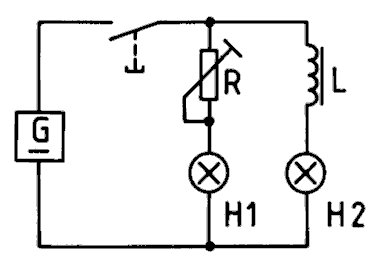
\includegraphics[scale=0.35]{Spule/Bilder/TC305.png}}%Frage
{leuchtet H1 zuerst.}%A
{leuchtet H2 zuerst.}%B
{leuchten H1 und H2 genau gleich schnell.}%C
{leuchtet H2 kurz auf und geht wieder aus. H1 leuchtet.}%D
{A}%Lösung

\mucho{9}{TC402}
{Ein Trafo liegt an 45 Volt und gibt 180 Volt ab. Seine Primärwicklung hat 150 Windungen. Wie groß ist seine Sekundärwindungszahl?}%Frage
{46 Windungen}%A
{30 Windungen}%B
{600 Windungen}%C
{850 Windungen}%D
{C: $\dfrac{N_1}{N_2} = \dfrac{U_1}{U_2}$; $N_2 = \dfrac{180V}{45V} \cdot 150$}%Lösung

\mucho{10}{TC403}
{Die Primärspule eines Übertragers hat die fünffache Anzahl von Windungen der Sekundärspule. Wie hoch ist die erwartete Sekundärspannung, wenn die Primärspule an eine 230-V-Stromversorgung angeschlossen wird?}%Frage
{46 Volt}%A
{9,2 Volt}%B
{23 Volt}%C
{1150 Volt}%D
{A: $\dfrac{N_1}{N_2} = \dfrac{U_1}{U_2}$; $U_2 = \dfrac{1}{5} \cdot 230V$}%Lösung

\mucho{11}{TC304}
{Das folgende Bild zeigt einen Kern, um den ein Kabel für den Bau einer Netzdrossel gewickelt ist. Der Kern sollte aus\\ 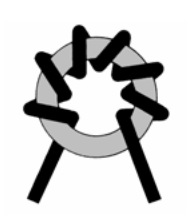
\includegraphics[scale=0.9]{Spule/Bilder/TC304.png}}%Frage
{Kunststoff bestehen.}%A
{Ferrit bestehen.}%B
{Stahl bestehen.}%C
{aus gut leitendem Material bestehen.}%D
{B}%Lösung

\mucho{12}{TC306}
{Mit zunehmender Frequenz}%Frage
{sinkt der Wechselstromwiderstand einer Spule.}%A
{sinkt der Wechselstromwiderstand einer Spule
bis zu einem Minimum und steigt dann wieder.}%B
{steigt der Wechselstromwiderstand einer Spule
bis zu einem Maximum und sinkt dann wieder.}%C
{steigt der Wechselstromwiderstand einer Spule.}%D
{D}%Lösung

%----------------------------
\newpage

\section*{Praktische Anwendung}

\subsection*{Spule wickeln}

% FIXME Foto einer eigenen Spule
\begin{wrapfigure}{r}{0.4\textwidth}
 \vspace{-10pt}
 \centering 
 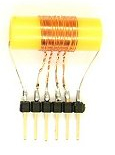
\includegraphics[scale=4]{Spule/Bilder/Spule_bau.jpg}
 %\caption{Bildunterschrift der Grafik.}
 %\label{fig:meine-Grafik}
 \vspace{-5pt}
\end{wrapfigure}

% Sollte auf Mehrband-RX hinführen - ist aber zu aufändig
% Für den ersten Versuch soll eine Spule mit insgesamt $25 $Windungen und vier
% Anzapfungen gewickelt werden. Als Wickelkörper soll eine 8 mm dickes und $3cm$
% langes Stück eines Trinkhalmes verwendet werden. Zwei Löcher im Abstand $1cm$
% helfen die Drahtenden zu fixieren. Es werden dann jeweils $5$ Windungen
% gewickelt, eine Schlaufe verdrillt und die folgenden Windungen aufgetragen. Die
% fertige Spule wird an einen Abschnitt Pfostenstecker mit sechs Kontakten
% gelötet. 

Für den ersten Versuch soll eine Spule aus $1 m$ Kupferlackdraht gewickelt
werden. Denkt daran beim Wickeln die Windungszahl zu zählen!

\begin{enumerate}
  \item Als Wickelkörper dient ein $8 mm$ dickes und $3cm$ langes Stück eines
    Trinkhalmes.
  \item Zwei Löcher im Abstand $1cm$ helfen die Drahtenden zu fixieren.
  \item Um die Kontakte der Spule frei zu legen, muss die aufgetragene
    Lackschicht abgeschabt oder mit einem Feuerzeug freigebrannt werden.
  \item Berechnet die Induktivität $L$ eurer Spule und messt mit dem
    LC-Messgerät nach.
\end{enumerate}

\loesung{Die Spule sollte um die $3-5 uH$ haben, damit der darauf aufbauende
KW-Empfänger-Versuch mit einem Schwingkreis um die $7 MHz$ klappt.}

\subsection*{Impedanz von C und L}

Wdh. Kondensator:

\begin{itemize}
    \item Erzeuge mit den Klinkenanschlusskabel und einem Signalgenerator
      Sinusschwingungen und finde heraus in welchem Bereich die Schwingungen
      noch deutlich hörbar sind.
    \item Schleife nun einen Koppelkondensator mit $C = 100 nF$ ein. Welche Unterschiede
      sind hörbar? \loesung{Hochpassverhalten}
    \item Berechne die Impedanz der Kondensators in den oberen und unteren
      Bereichen der Hörschwelle.
    \item Zusatzaufgabe: Was passiert mit einem Rechtecksignal?
\end{itemize}

% TODO Induktivität/Kapazität als Energiespeicher:
%      * siehe Experiment TC305
%      * Glimmlampen
%      * mit Dioden antiparallel?

Spule:

\begin{itemize}
  \item Wiederholt das o.g. Experiment mit eurer Spule -- was fällt euch auf?
  \item Wiederholt das o.g. Experiment noch einmal mit einer geg. Spule -- hier
    reicht das Messen der Impedanz % FIXME
\end{itemize}

\loesung{Ziel in diesem Teil ist es herauszufinden, dass es unglaubliche
Windugszahlen bei Spulen erfordert um etwas im niederfrequenten Bereich zu
erreichen.}

% DONE Spannungsteilerversuch mit 1 Ohm und Induktivität von bis zu 20 uH
%      fehlgeschlagen :-( Allein die Übergangswiderstände machen schon zu viel aus
% TODO einfaches Audiofilter als Notch?
% TODO Induktionsversuch a la Trafo?



\chapter{Der Schwingkreis}
%\begin{wrapfigure}[0]{r}[-2.5cm]{3cm}
% \vspace{-6cm}
% \includegraphics[scale=0.4]{Schwingkreis/Bilder/schwingkreis.png}
% \vspace{-6cm}
%\end{wrapfigure}

\section*{Theorie- und Prüfungsfragen} 

\mucho{1}{TD203}
{Was ist im Resonanzfall bei der Reihenschaltung einer Induktivität mit einer Kapazität erfüllt?}%Frage
{Der Betrag des induktiven Widerstands ist dann gleich dem Betrag des kapazitiven Widerstands.}%A
{Der Wert des Verlustwiderstands der Spule ist dann gleich dem Wert des Verlustwiderstands des Kondensators.}%B
{Die Größe des elektrischen Feldes in der Spule ist dann gleich der Größe des elektrischen Feldes im Kondensators.}%C
{Die Größe des magnetischen Feldes in der Spule ist dann gleich der Größe des magnetischen Feldes im Kondensator.}%D
{A}%Lösung

\mucho{2}{TD209}
{Welche Resonanzfrequenz hat die Parallelschaltung einer Spule von 2 $\mu H$ mit einem Kondensator von 60 $pF$ und einem Widerstand von 10$k\Omega$?}%Frage
{145,288kHz}%A
{1,45288MHz}%B
{14,5288MHz}%C
{145,288 MHz}%D
{C \hspace{3em} $f_0 = \frac{1}{2 \pi \sqrt{L C}}$}%Lösung

\mucho{3}{TD206}
{ Wie ändert sich die Resonanzfrequenz eines Schwingkreises, wenn
1. die Spule mehr Windungen erhält, 2. die Länge der Spule durch Zusammenschieben der Drahtwicklung verringert wird, 3. ein Kupferkern in das Innere der Spule gebracht wird?}%Frage
{Die Resonanzfrequenz wird bei 1. und 2. kleiner und bei 3. größer.}%A
{Die Resonanzfrequenz wird in allen drei Fällen kleiner.}%B
{Die Resonanzfrequenz wird bei 1. kleiner und bei 2. und 3. größer.}%C
{Die Resonanzfrequenz wird bei 1. und 2. größer und bei 3. kleiner.}%D
{A}%Lösung


\mucho{4}{TD201}
{Der Impedanzfrequenzgang in der Abbildung zeigt die Kennlinie\\ 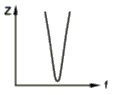
\includegraphics[scale=0.5]{Schwingkreis/Bilder/TD201.png}}%Frage
{eines Serienschwingkreises.}%A
{eines Parallelschwingkreises.}%B
{einer Induktivität.}%C
{einer Kapazität.}%D
{A}%Lösung

\vspace*{0.65cm}

\mucho{5}{TD202}
{Der Impedanzfrequenzgang in der Abbildung zeigt die Kennlinie\\
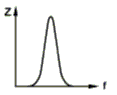
\includegraphics[scale=0.5]{Schwingkreis/Bilder/TD202.png}}%Frage
{eines Serienschwingkreises.}%A
{eines Parallelschwingkreises.}%B
{einer Induktivität.}%C
{einer Kapazität.}
{B}%Lösung

\aufgabentext{
	\begin{enumerate}
	\item[6] Um welche Schaltungen handelt es sich in folgender Abbildung.
	\end{enumerate}
	\loesung{1 Reihenschwingkreis, 2 Parallelschwingkreis, 3 Tiefpass, 4 Hochpass, 5 Bandpass, 6 Saugkreis, 7 Sperrkreis }
	}

\begin{figure}[H]
	\centering
	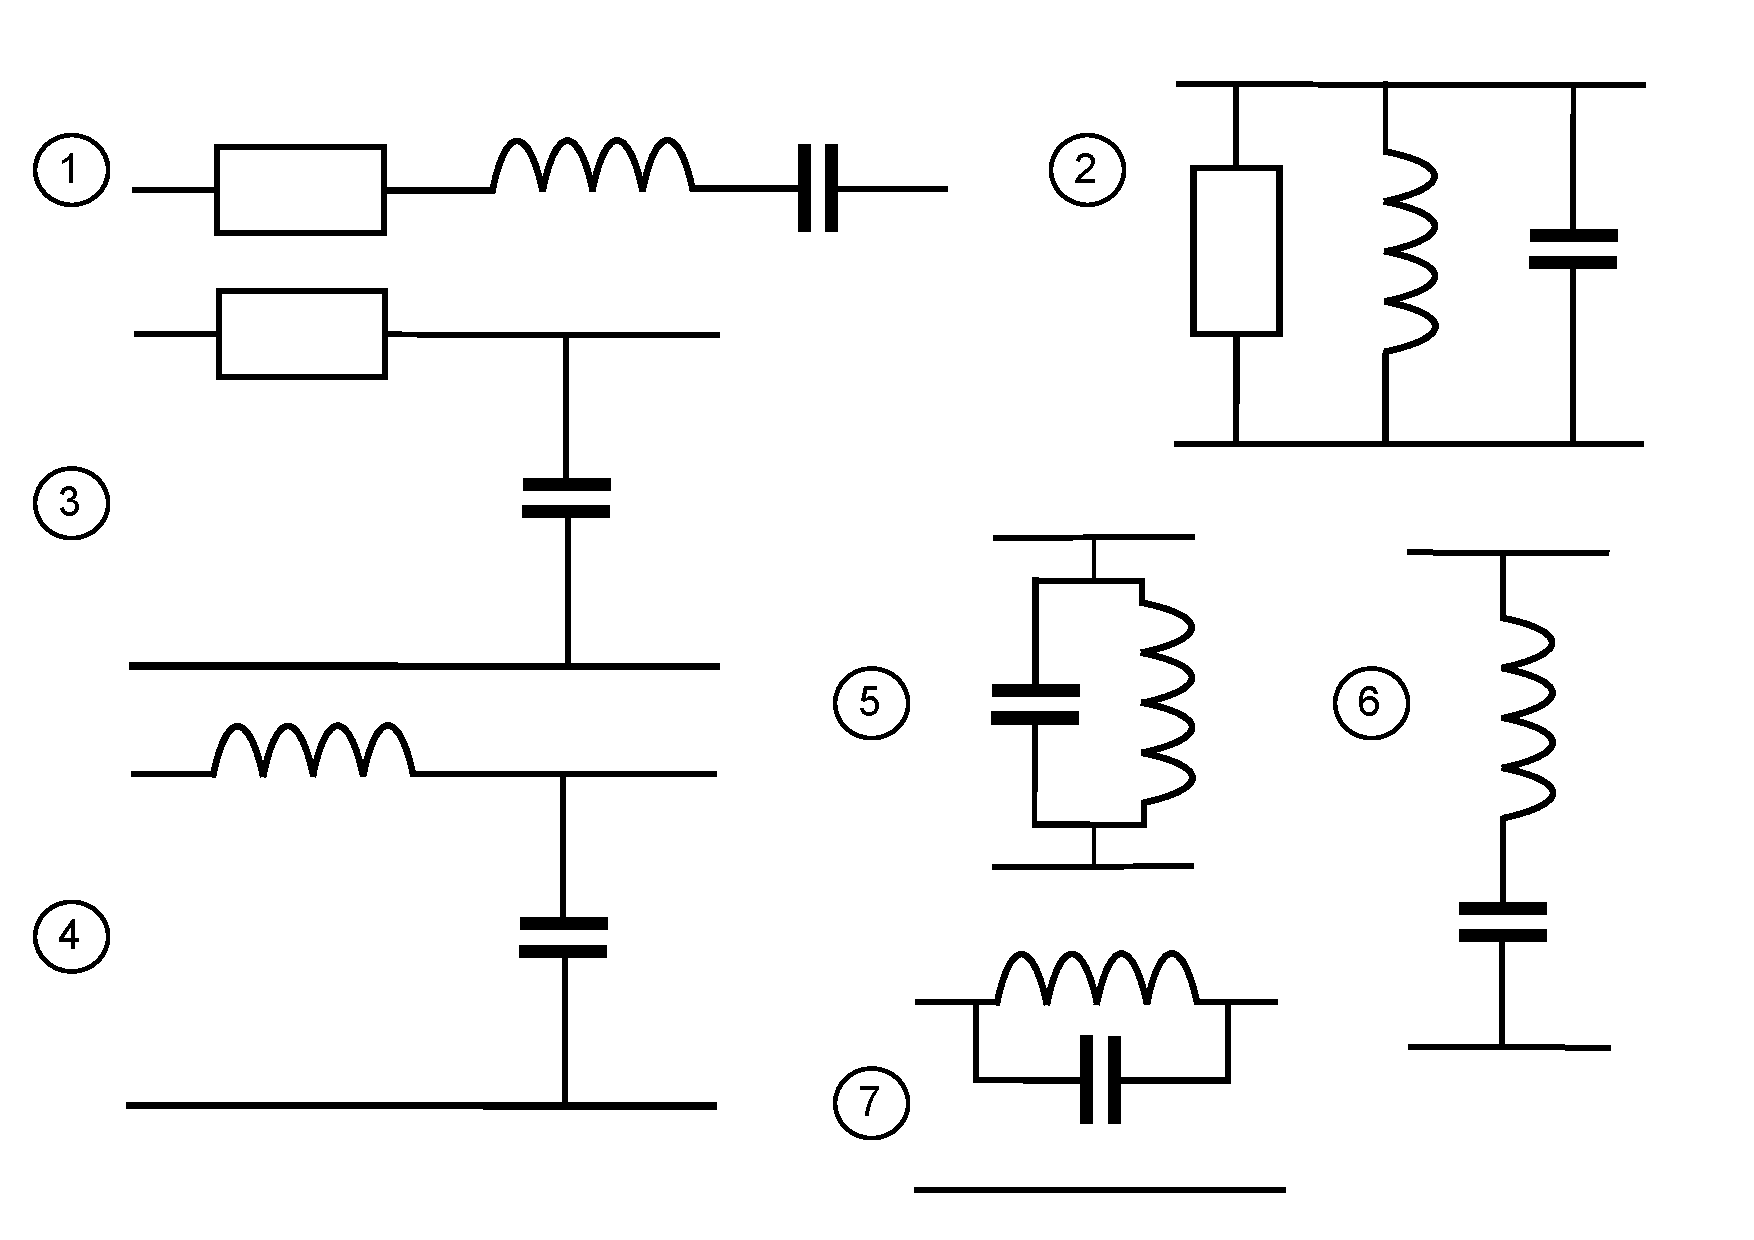
\includegraphics[scale=0.5]{Schwingkreis/Bilder/Filterschaltungen.pdf}
	\end{figure}

\mucho{7}{TD213}
{Welche Grenzfrequenz ergibt sich bei einem RC-Tiefpass mit einem Widerstand von 10$k\Omega$ und einem Kondensator von 50$nF$?}%Frage
{0,32$Hz$}%A
{318$Hz$}%B
{421$Hz$}%C
{318$kHz$}%D
{B \hspace{3em} $f_g = \frac{1}{2 \pi R C}$}%Lösung

\section*{Praxis}

\subsection*{Vorbereitung}

Seht euch die Pin-Belegung des Raspberry Pi (siehe Abbildung \ref{rpi}) sowie
die zu layoutende Schaltung für den 70cm-Tiefpassfilter (siehe Abbildung
\ref{70cmLP}) an.

\begin{figure}[H]
    \centering
    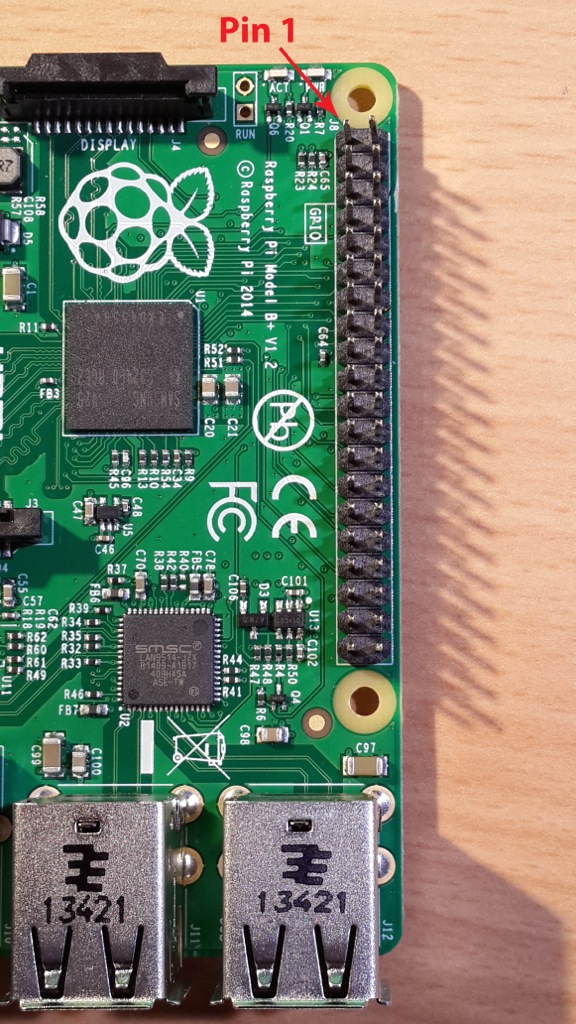
\includegraphics[height=0.4\textheight]{Schwingkreis/Bilder/B_plus_hdr_sm.jpg}
    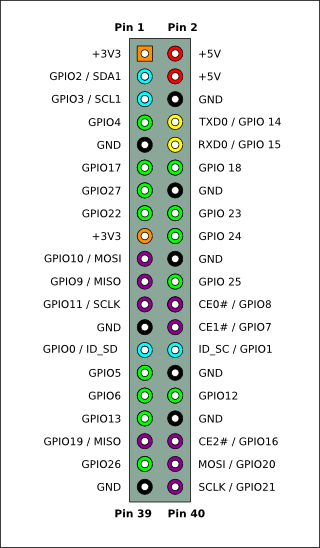
\includegraphics[height=0.4\textheight]{Schwingkreis/Bilder/Pi-GPIO-header.png}
    \caption{Connector pinout (P1 Header) -- Models B+, B2}
    \label{rpi}
    %FIXME Abbildungs-Quellenverzeichnis \url{http://elinux.org/RPi_Low-level_peripherals#Model_A.2B.2C_B.2B_and_B2}
\end{figure}

\begin{figure}[H]
    \centering
    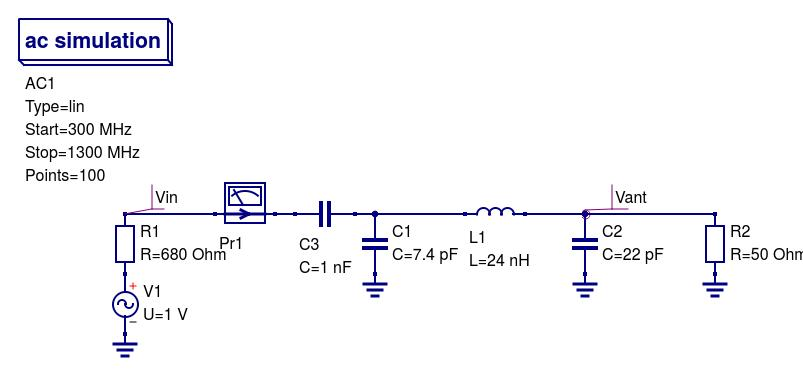
\includegraphics[width=1\textwidth]{Schwingkreis/Bilder/70cmLP500Ohm.jpg}
    \caption{Schaltung des 70cm-Tiefpassfilters aus Qucs}
    \label{70cmLP}
\end{figure}

\subsection*{Fritzing}

\subsubsection{Schematic View}

Bauteile aus den \emph{Core Parts} hinzufügen:

\begin{itemize}
    \item  Basic
    \begin{itemize}
        \item Resistor $680 \Omega$ (THT)
        \item Inductor $22 nH$ (SMD 1206)
        \item Ceramic Capacitor $1 nF$ (THT)
        \item Ceramic Capacitor $22 pF$ (THT)
    \end{itemize}
    \item  Input
    \begin{itemize}
        \item Variable Capacitor $2.1-10 pF$ (THT, $3.81mm$ pin spacing)
        \item Antenna (Wire soldering point)
    \end{itemize}
    \item Connection
    \begin{itemize}
        \item Generic female header (THT, 2x10, flip horizontal)
    \end{itemize}
    \item Schematic View
    \begin{itemize}
        \item Ground
    \end{itemize}
\end{itemize}

Nun können die Bauteile entsprechend des Schaltplanes verdrahtet werden.
\textbf{Hinweis}: Die Pin-Zählung des \emph{Generic female header} stimmt nicht
mit der des Raspberry Pi überein.

\begin{itemize}
    \item GPIO = Pin 16
    \item GND = Pin 17
\end{itemize}

\subsubsection{PCB View}

\begin{itemize}
    \item PCB ändern auf One Layer \& Fäche ca. $30x30mm$
    \item Bauteile anordnen (THT-Bauteile auf Vorderseite, SMD auf Unterseite)
    \item Leitungen ziehen
    \item optional: Copper Fill Blocker \& Silkscreen Text
    \item Rechtsklick auf einen Ground Pin: "`Set Ground Fill Seed"'
    \item Menü $\rightarrow$ Routing $\rightarrow$ Ground Fill
\end{itemize}

\subsubsection{Zusatzaufgaben}

\begin{itemize}
    \item Antennenanschluss auf folgende MCX-Buchse umbauen: \\
          \url{http://www.reichelt.de/index.html?ARTICLE=152523}
    \item Testboard mit verschiedenen PCB-Spulen um ~24 nH erstellen, da typ. 2-3\% Abweichung. \\
          Berechnungsgrundlagen mit Online calculator:\\
          \url{http://coil32.net/pcb-coil.html}\\
          alternative Formen: \\
          \url{http://www.circuits.dk/calculator_planar_coil_inductor.htm}
\end{itemize}


\chapter{Die Diode}


\begin{wrapfigure}[0]{r}[-2cm]{4cm}
 \vspace{-5cm}
 %\centering 
 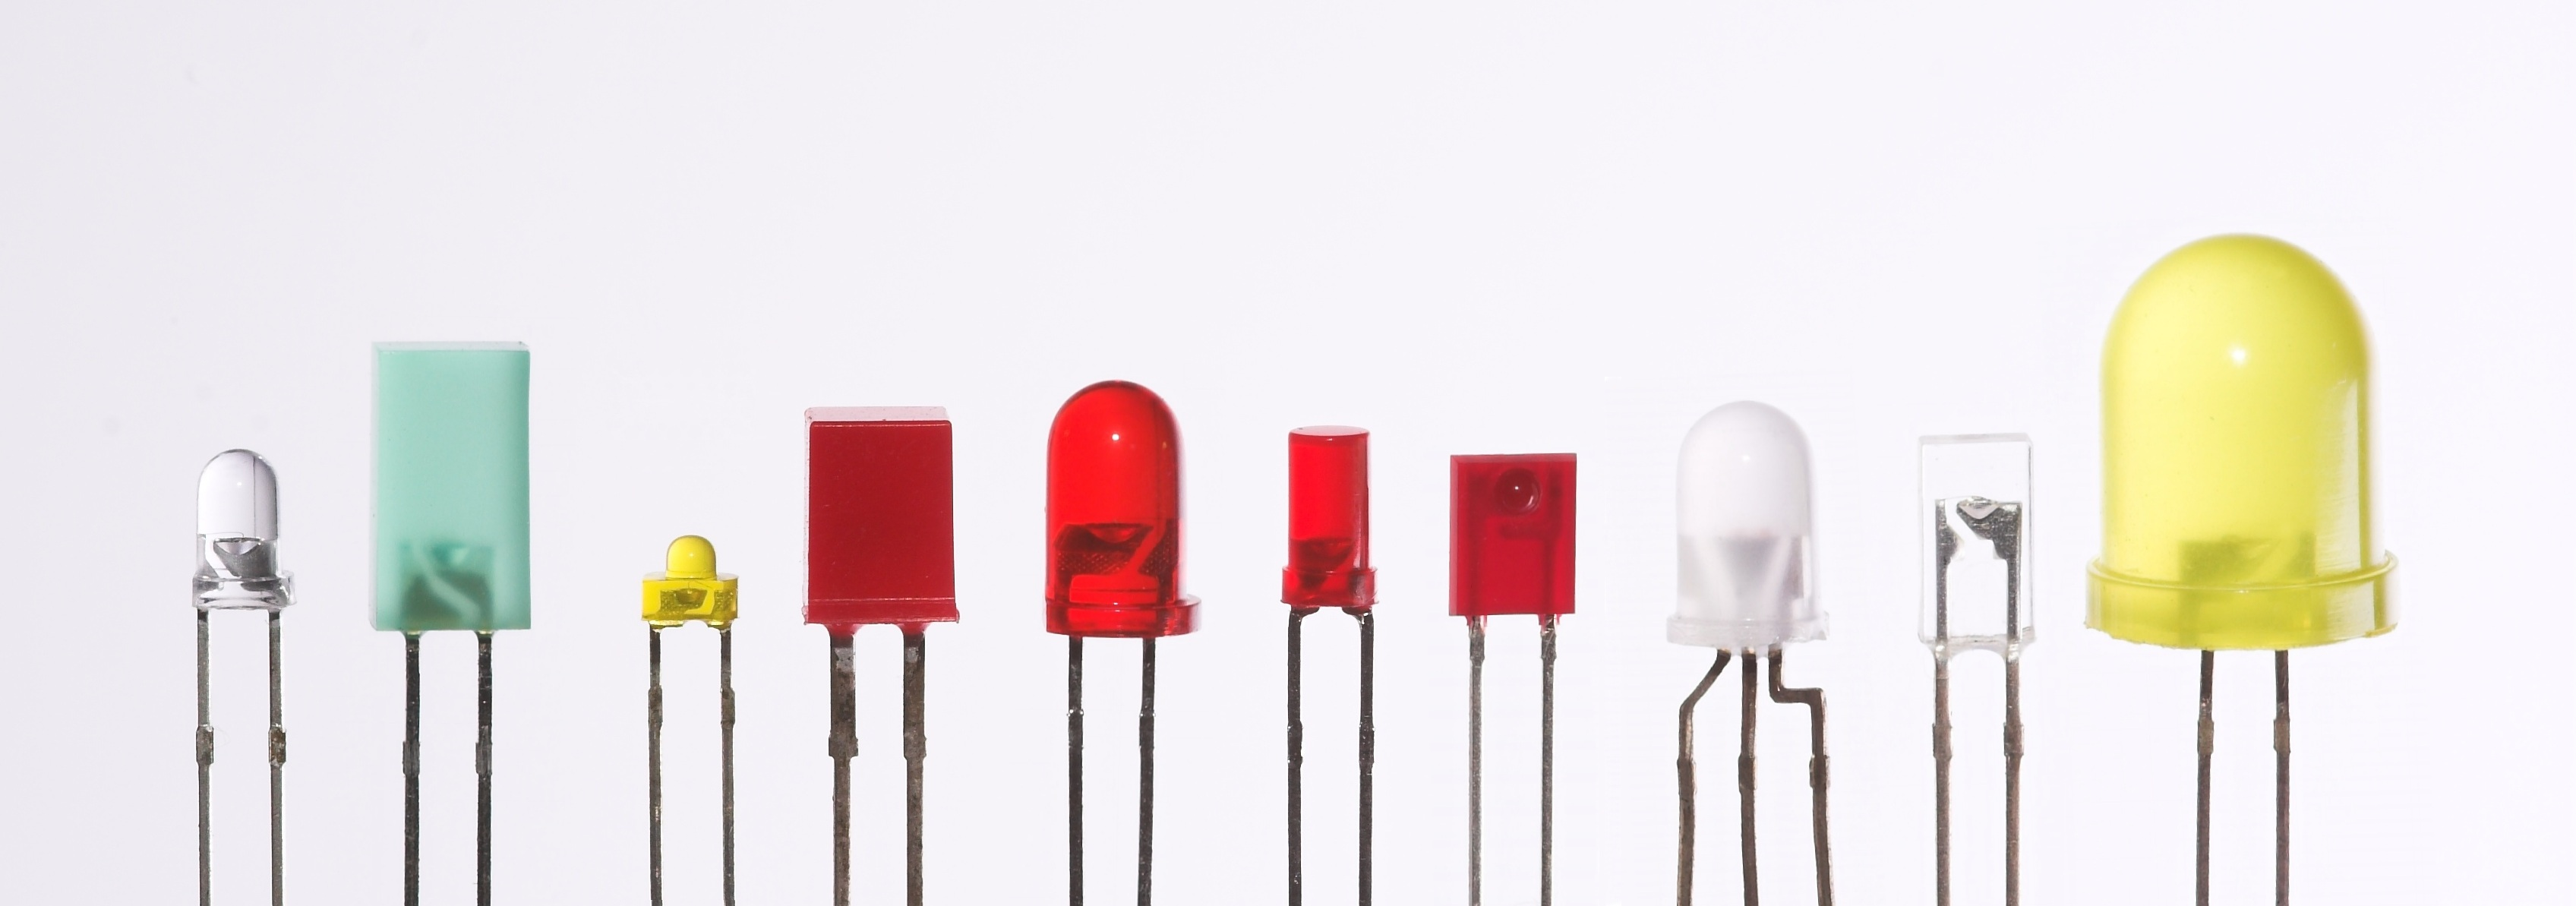
\includegraphics[scale=0.25]{Diode/Bilder/Verschiedene_LEDs.jpg}
 %\caption{Bildunterschrift der Grafik.}
 %\label{fig:meine-Grafik}
 \vspace*{-5cm}
\end{wrapfigure}


\section*{Theorie- und Prüfungsfragen} 

\subsection*{Dotierung}

\begin{enumerate}
	\itemsep1pt\parskip0pt\parsep0pt
	\item[1] Was bedeutet der Begriff Dotierung?
        \loesung{\textbf{Dotierung} bezeichnet in der Halbleitertechnik das
        einbringen von Fremdatomen in ein Grundmaterial zur Veränderung der
        elektrischen Leitfähigkeit.}
\end{enumerate}

\begin{enumerate}
\item[2] \emph{\textbf{TB105}}    Was verstehen Sie unter Halbleitermaterialien? Einige Stoffe wie z.B. ...
	\begin{enumerate}
	\itemsep1pt\parskip0pt\parsep0pt
		\item[A] Silizium, Germanium sind in reinem Zustand gute Isolatoren. Durch geringfügige Zusätze von geeigneten anderen Stoffen werden sie jedoch zu Leitern.
		\item[B] Silizium, Germanium sind in reinem Zustand gute Isolatoren. Durch geringfügige Zusätze von geeigneten anderen Stoffen nimmt jedoch ihre Leitfähigkeit ab.
		\item[C]  Indium oder Magnesium sind in reinem Zustand gute Isolatoren. Durch geringfügige Zusätze von geeigneten anderen Stoffen werden sie jedoch zu Leitern.
		\item[D] Silizium, Germanium sind in trockenem Zustand gute Elektrolyten. Durch geringfügige Zusätze von Wismut oder Tellur kann man daraus entweder N-leitendes oder P-leitendes Material für Anoden bzw. Katoden von Halbleiterbauelementen herstellen.
		\loesung{Lösung A}
	\end{enumerate}
\end{enumerate}

\begin{enumerate}
\item[3] \emph{\textbf{TC501}}    P-dotiertes Halbleitermaterial ist solches, das mit einem zusätzlichen Stoff versehen wurde, der
	\begin{enumerate}
	\itemsep1pt\parskip0pt\parsep0pt
		\item[A] mehr als vier Valenzelektronen enthält.
		\item[B] genau vier Valenzelektronen enthält.
		\item[C] weniger als vier Valenzelektronen enthält.
		\item[D] keine Valenzelektronen enthält.
		 \loesung{Lösung C}
	\end{enumerate}
\end{enumerate}


\begin{enumerate}
\item[4] \emph{\textbf{TC502}}   N-leitendes Halbleitermaterial ist gekennzeichnet durch
	\begin{enumerate}
	\itemsep1pt\parskip0pt\parsep0pt
		\item[A] Überschuss an freien Elektronen.
		\item[B] das Fehlen von Dotierungsatomen.
		\item[C] das Fehlen von Atomen im Gitter des Halbleiterkristalls.
		\item[D] bewegliche Elektronenlücken.
		\loesung{Lösung A}
	\end{enumerate}
\end{enumerate}


\begin{enumerate}
\item[5] \emph{\textbf{TC503}}  Ein in Durchlassrichtung betriebener PN-Übergang ermöglicht
	\begin{enumerate}
	\itemsep1pt\parskip0pt\parsep0pt
		\item[A] den Stromfluss von N nach P.
		\item[B] den Stromfluss von P nach N.
		\item[C] keinen Stromfluss.
		\item[D] den Elektronenfluss von P nach N.
		\loesung{Lösung B}
	\end{enumerate}
\end{enumerate}


\subsection*{Die Diode}

\begin{enumerate}
\itemsep1pt\parskip0pt\parsep0pt
\item[6] Skizziere das Schaltzeichen einer Diode und markiere die Anode, die Kathode und die jeweilige Dotierung.
    \loesung{
    \begin{figure}[H]
    \centering 
    % Graphic for TeX using PGF
% Title: /home/stole/Dokumente/git/afutub-kurs/Praxisskript/Diode/Schaltungen/Diode.dia
% Creator: Dia v0.97.3
% CreationDate: Mon Nov 16 20:36:17 2015
% For: stole
% \usepackage{tikz}
% The following commands are not supported in PSTricks at present
% We define them conditionally, so when they are implemented,
% this pgf file will use them.
\ifx\du\undefined
  \newlength{\du}
\fi
\setlength{\du}{15\unitlength}
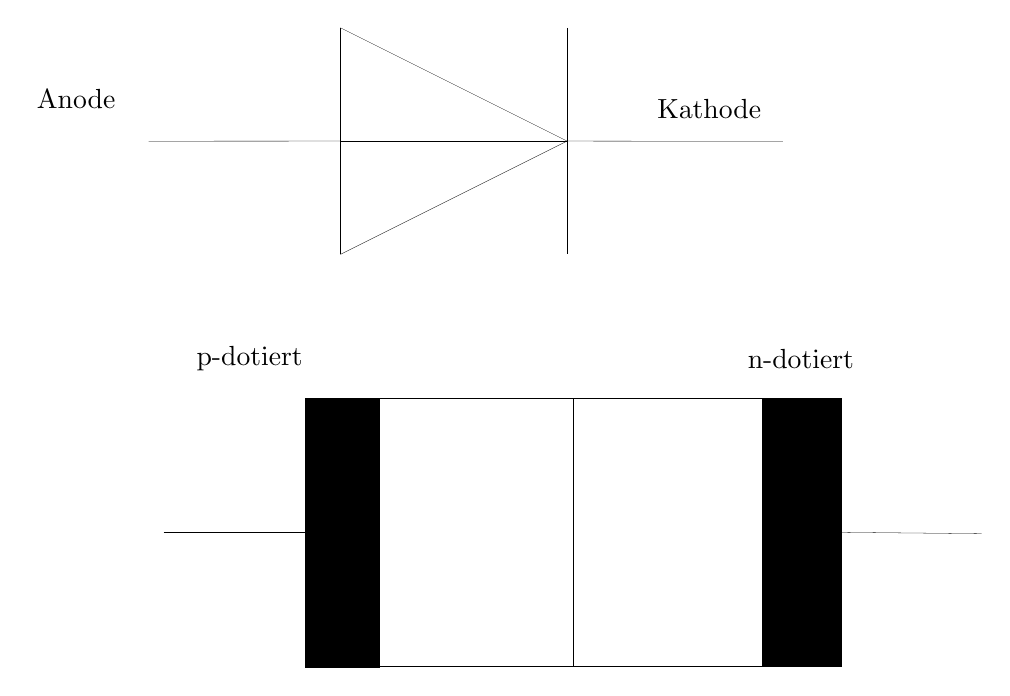
\begin{tikzpicture}
\pgftransformxscale{1.000000}
\pgftransformyscale{-1.000000}
\definecolor{dialinecolor}{rgb}{0.000000, 0.000000, 0.000000}
\pgfsetstrokecolor{dialinecolor}
\definecolor{dialinecolor}{rgb}{1.000000, 1.000000, 1.000000}
\pgfsetfillcolor{dialinecolor}
\pgfsetlinewidth{0.100000\du}
\pgfsetdash{}{0pt}
\pgfsetdash{}{0pt}
\pgfsetbuttcap
\pgfsetmiterjoin
\pgfsetbuttcap
\pgfsetmiterjoin
\pgfsetdash{}{0pt}
\definecolor{dialinecolor}{rgb}{0.000000, 0.000000, 0.000000}
\pgfsetstrokecolor{dialinecolor}
\draw (15.422302\du,-15.899999\du)--(15.422302\du,-13.022298\du);
\pgfsetbuttcap
\pgfsetmiterjoin
\pgfsetdash{}{0pt}
\definecolor{dialinecolor}{rgb}{0.000000, 0.000000, 0.000000}
\pgfsetstrokecolor{dialinecolor}
\draw (15.422302\du,-13.022298\du)--(18.300002\du,-14.461149\du);
\pgfsetbuttcap
\pgfsetmiterjoin
\pgfsetdash{}{0pt}
\definecolor{dialinecolor}{rgb}{0.000000, 0.000000, 0.000000}
\pgfsetstrokecolor{dialinecolor}
\draw (15.422302\du,-15.899999\du)--(18.300002\du,-14.461149\du);
\pgfsetbuttcap
\pgfsetmiterjoin
\pgfsetdash{}{0pt}
\definecolor{dialinecolor}{rgb}{0.000000, 0.000000, 0.000000}
\pgfsetstrokecolor{dialinecolor}
\draw (15.422302\du,-14.461149\du)--(18.300002\du,-14.461149\du);
\pgfsetbuttcap
\pgfsetmiterjoin
\pgfsetdash{}{0pt}
\definecolor{dialinecolor}{rgb}{0.000000, 0.000000, 0.000000}
\pgfsetstrokecolor{dialinecolor}
\draw (18.300002\du,-15.899999\du)--(18.300002\du,-13.022298\du);
\pgfsetlinewidth{0.100000\du}
\pgfsetdash{}{0pt}
\pgfsetdash{}{0pt}
\pgfsetbuttcap
{
\definecolor{dialinecolor}{rgb}{0.000000, 0.000000, 0.000000}
\pgfsetfillcolor{dialinecolor}
% was here!!!
\definecolor{dialinecolor}{rgb}{0.000000, 0.000000, 0.000000}
\pgfsetstrokecolor{dialinecolor}
\draw (18.300002\du,-14.461149\du)--(21.040301\du,-14.459230\du);
}
\pgfsetlinewidth{0.100000\du}
\pgfsetdash{}{0pt}
\pgfsetdash{}{0pt}
\pgfsetbuttcap
{
\definecolor{dialinecolor}{rgb}{0.000000, 0.000000, 0.000000}
\pgfsetfillcolor{dialinecolor}
% was here!!!
\definecolor{dialinecolor}{rgb}{0.000000, 0.000000, 0.000000}
\pgfsetstrokecolor{dialinecolor}
\draw (12.987653\du,-14.460276\du)--(15.422302\du,-14.461149\du);
}
% setfont left to latex
\definecolor{dialinecolor}{rgb}{0.000000, 0.000000, 0.000000}
\pgfsetstrokecolor{dialinecolor}
\node[anchor=west] at (11.448825\du,-14.995418\du){Anode};
% setfont left to latex
\definecolor{dialinecolor}{rgb}{0.000000, 0.000000, 0.000000}
\pgfsetstrokecolor{dialinecolor}
\node[anchor=west] at (19.327825\du,-14.872736\du){Kathode};
\pgfsetlinewidth{0.100000\du}
\pgfsetdash{}{0pt}
\pgfsetdash{}{0pt}
\pgfsetmiterjoin
\definecolor{dialinecolor}{rgb}{1.000000, 1.000000, 1.000000}
\pgfsetfillcolor{dialinecolor}
\fill (14.976770\du,-11.192971\du)--(14.976770\du,-7.792972\du)--(18.376770\du,-7.792972\du)--(18.376770\du,-11.192971\du)--cycle;
\definecolor{dialinecolor}{rgb}{0.000000, 0.000000, 0.000000}
\pgfsetstrokecolor{dialinecolor}
\draw (14.976770\du,-11.192971\du)--(14.976770\du,-7.792972\du)--(18.376770\du,-7.792972\du)--(18.376770\du,-11.192971\du)--cycle;
\pgfsetlinewidth{0.100000\du}
\pgfsetdash{}{0pt}
\pgfsetdash{}{0pt}
\pgfsetmiterjoin
\definecolor{dialinecolor}{rgb}{1.000000, 1.000000, 1.000000}
\pgfsetfillcolor{dialinecolor}
\fill (18.376770\du,-11.192970\du)--(18.376770\du,-7.792971\du)--(21.776770\du,-7.792971\du)--(21.776770\du,-11.192970\du)--cycle;
\definecolor{dialinecolor}{rgb}{0.000000, 0.000000, 0.000000}
\pgfsetstrokecolor{dialinecolor}
\draw (18.376770\du,-11.192970\du)--(18.376770\du,-7.792971\du)--(21.776770\du,-7.792971\du)--(21.776770\du,-11.192970\du)--cycle;
\pgfsetlinewidth{0.100000\du}
\pgfsetdash{}{0pt}
\pgfsetdash{}{0pt}
\pgfsetbuttcap
{
\definecolor{dialinecolor}{rgb}{0.000000, 0.000000, 0.000000}
\pgfsetfillcolor{dialinecolor}
% was here!!!
\definecolor{dialinecolor}{rgb}{0.000000, 0.000000, 0.000000}
\pgfsetstrokecolor{dialinecolor}
\draw (13.176770\du,-9.492971\du)--(14.976770\du,-9.492972\du);
}
\pgfsetlinewidth{0.100000\du}
\pgfsetdash{}{0pt}
\pgfsetdash{}{0pt}
\pgfsetmiterjoin
\definecolor{dialinecolor}{rgb}{0.000000, 0.000000, 0.000000}
\pgfsetfillcolor{dialinecolor}
\fill (14.976770\du,-11.192971\du)--(14.976770\du,-7.778107\du)--(15.911899\du,-7.778107\du)--(15.911899\du,-11.192971\du)--cycle;
\definecolor{dialinecolor}{rgb}{0.000000, 0.000000, 0.000000}
\pgfsetstrokecolor{dialinecolor}
\draw (14.976770\du,-11.192971\du)--(14.976770\du,-7.778107\du)--(15.911899\du,-7.778107\du)--(15.911899\du,-11.192971\du)--cycle;
\pgfsetlinewidth{0.100000\du}
\pgfsetdash{}{0pt}
\pgfsetdash{}{0pt}
\pgfsetmiterjoin
\definecolor{dialinecolor}{rgb}{0.000000, 0.000000, 0.000000}
\pgfsetfillcolor{dialinecolor}
\fill (20.776770\du,-11.192971\du)--(20.776770\du,-7.792971\du)--(21.776770\du,-7.792971\du)--(21.776770\du,-11.192971\du)--cycle;
\definecolor{dialinecolor}{rgb}{0.000000, 0.000000, 0.000000}
\pgfsetstrokecolor{dialinecolor}
\draw (20.776770\du,-11.192971\du)--(20.776770\du,-7.792971\du)--(21.776770\du,-7.792971\du)--(21.776770\du,-11.192971\du)--cycle;
% setfont left to latex
\definecolor{dialinecolor}{rgb}{0.000000, 0.000000, 0.000000}
\pgfsetstrokecolor{dialinecolor}
\node[anchor=west] at (13.476772\du,-11.692970\du){p-dotiert};
% setfont left to latex
\definecolor{dialinecolor}{rgb}{0.000000, 0.000000, 0.000000}
\pgfsetstrokecolor{dialinecolor}
\node[anchor=west] at (20.476772\du,-11.692970\du){n-dotiert};
\pgfsetlinewidth{0.100000\du}
\pgfsetdash{}{0pt}
\pgfsetdash{}{0pt}
\pgfsetbuttcap
{
\definecolor{dialinecolor}{rgb}{0.000000, 0.000000, 0.000000}
\pgfsetfillcolor{dialinecolor}
% was here!!!
\definecolor{dialinecolor}{rgb}{0.000000, 0.000000, 0.000000}
\pgfsetstrokecolor{dialinecolor}
\draw (21.776770\du,-9.492971\du)--(23.565624\du,-9.475251\du);
}
\end{tikzpicture}

    \end{figure}
    }
\item[7] Skizziere die Strom-Spannungskennlinie und markieren den Durchlassbereich, den Sperrbereich und den Durchbruchbereich.
	\loesung{
	\begin{figure}[H]
    \centering 
    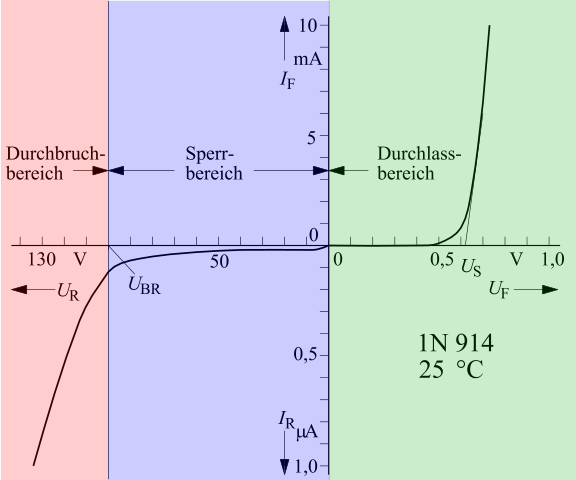
\includegraphics[scale=0.5]{Diode/Bilder/Kennlinie_Diode.png}
    \end{figure}
    }
\end{enumerate}

\mucho{8}{TC504}
{Eine in Sperrrichtung betriebene Diode hat}%Frage
{einen hohen Widerstand.}%A
{eine hohe Kapazität.}%B
{eine geringe Impedanz.}%C
{eine hohe Induktivität.}%D
{A}%Lösung

\mucho{9}{TC508}
{Wozu dient die folgende Schaltung?\\ 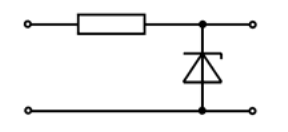
\includegraphics[scale=0.63]{Diode/Bilder/TC508.png}}%Frage
{zur Signalbegrenzung.}%A
{zur Spannungsstabilisierung.}%B
{als Leuchtanzeige.}%C
{zur Stromgewinnung.}%D
{B}%Lösung

\mucho{10}{TC505}
{Die Auswahlantworten enthalten Silizium-Dioden mit unterschiedlichen Arbeitspunkten. Bei welcher Antwort befindet sich die Diode in leitendem Zustand?}%Frage
{$-2,6V $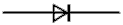
\includegraphics[scale=0.5]{Diode/Bilder/Diode_r.png} $-2,0V$}%A
{$~~~~15V$ 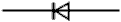
\includegraphics[scale=0.5]{Diode/Bilder/Diode_l.png} $~~~9V$}%B
{$~~0,7V$ 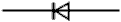
\includegraphics[scale=0.5]{Diode/Bilder/Diode_l.png} $1,3V$}%C
{$~~3,4V$ 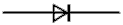
\includegraphics[scale=0.5]{Diode/Bilder/Diode_r.png} $4,0V$}%D
{C}%Lösung

\mucho{11}{TC506}
{Die Auswahlantworten enthalten Silizium-Dioden mit unterschiedlichen Arbeitspunkten. Bei welcher Antwort befindet sich die Diode in leitendem Zustand?}%Frage
{$~~5,3V $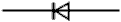
\includegraphics[scale=0.5]{Diode/Bilder/Diode_l.png} $4,7V$}%A
{$~~15V$ 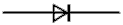
\includegraphics[scale=0.5]{Diode/Bilder/Diode_r.png} $18V$}%B
{$3,9V$ 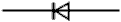
\includegraphics[scale=0.5]{Diode/Bilder/Diode_l.png} $3,2V$}%C
{$-2V$ 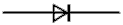
\includegraphics[scale=0.5]{Diode/Bilder/Diode_r.png} $-2,6V$}%D
{D}%Lösung

\mucho{12}{TC509}
{Wozu dient die folgende Schaltung?\\ 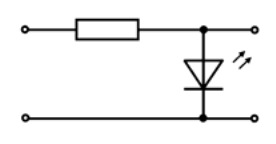
\includegraphics[scale=0.63]{Diode/Bilder/TC509.png}}%Frage
{zur Signalbegrenzung.}%A
{als Leuchtanzeige.}%B
{zur Stromgewinnung.}%C
{zur Spannungsstabilisierung.}%D
{B}%Lösung

\mucho{13}{TC507}
{Wie verhält sich die Kapazität einer Kapazitätsdiode (Varicap)?}%Frage
{Sie nimmt mit abnehmender Sperrspannung zu.}%A
{Sie erhöht sich mit zunehmender Durchlassspannung.}%B
{Sie nimmt mit zunehmender Sperrspannung zu.}%C
{Sie erhöht sich mit zunehmendem Durchlassstrom.}%D
{B}%Lösung


\chapter{Der Bipolar-Transistor}


\begin{wrapfigure}[2]{r}[-1cm]{4cm}
 \vspace{-6cm}
  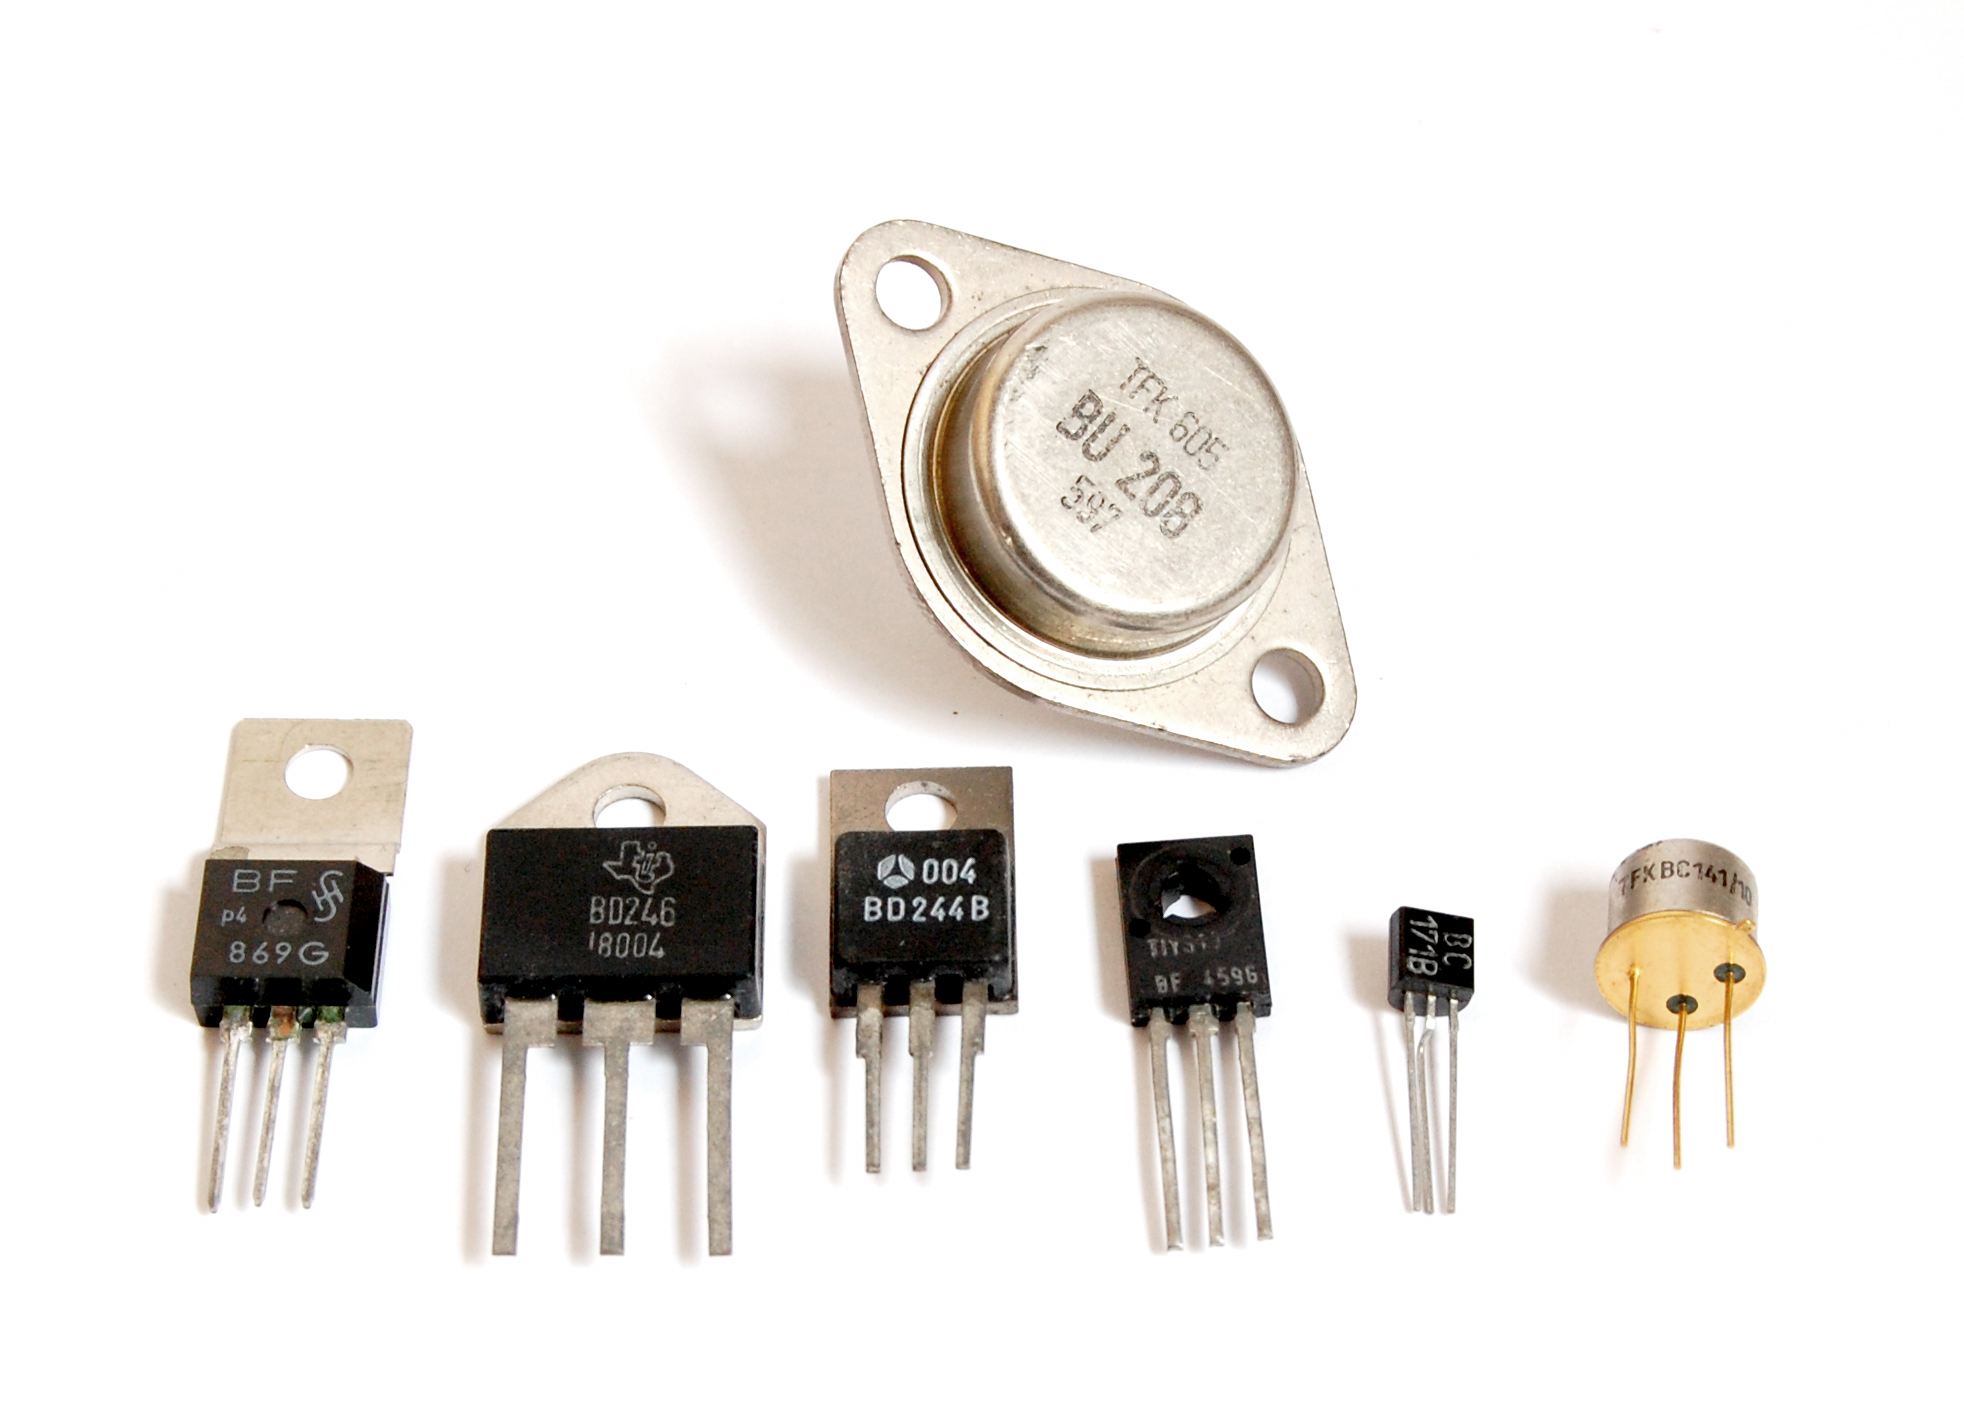
\includegraphics[scale=0.4]{Transistor/Bilder/Transistors-white.jpg}
 \vspace{-6cm}
\end{wrapfigure}

\section{Theorie- und Prüfungsfragen}

~~~~~~

\begin{enumerate}
\itemsep1pt\parskip0pt\parsep0pt
\item[i] Skizzieren Sie die Schaltzeichen eines NPN- und eines PNP-Transistors. Beschriften Sie entsprechend die Anschlüsse.
\item[ii] Zeichnen Sie das Ersatzschaltbild aus zwei Dioden für den NPN- und den PNP-Transistor.
\end{enumerate}

\begin{enumerate} 
\item[iii] \emph{\textbf{TC605}} Welche Kollektorspannungen haben NPN- und PNP-Transistoren?
	\begin{enumerate}
	\itemsep1pt\parskip0pt\parsep0pt
		\item[a] NPN- und PNP-Transistoren benötigen negative Kollektorspannungen.
		\item[b] PNP-Transistoren benötigen positive, NPN-Transistoren negative Kollektorspannung.
		\item[c] PNP- und NPN-Transistoren benötigen positive Kollektorspannungen.
		\item[d] NPN-Transistoren benötigen positive, PNP-Transistoren negative Kollektorspannungen.
	\end{enumerate}
\end{enumerate}

\loesung{	
	iii d
}

\begin{enumerate} 
\item[iv] \emph{\textbf{TC602}}  Das Verhältnis von Kollektorstrom zum Basisstrom eines Transistors liegt üblicherweise im Bereich von
	\begin{enumerate}
	\itemsep1pt\parskip0pt\parsep0pt
		\item[a] 1 zu 50 bis 1 zu 100.
		\item[b] 10 zu 1 bis 900 zu 1.
		\item[c] 1000 zu 1 bis 5000 zu 1.
		\item[d] 1 zu 100 bis 1 zu 500.
	\end{enumerate}
\end{enumerate}

\loesung{	
	iv b
}

\section{Praktische Anwendung}

\subsection[Der Bipolar-Transistor als Schalter]{Transistorschaltung 01 - Der Bipolar-Transistor als Schalter}

\begin{itemize}
\itemsep1pt\parskip0pt\parsep0pt
\item Schauen Sie sich den Bipolar-Transistor als Bauteil an und ordnen Sie die Bezeichnungen Kollektor, Basis und Emitter den einzelnen Beinchen zu.
\item Bauen Sie folgende Transistor-Schaltung auf (Abbildung \ref{s01}). 
\item Legen Sie die Versorgungsspannung an die Schaltung an.
\item Entfernen Sie unter Last die Leuchtdiode 1. Welche Auswirkungen hat das auf die Schaltung und warum?
\item \textbf{Zusatz:} Ersetzen Sie die Led durch einen Lautsprecher? Was passiert und warum?
\end{itemize}

\begin{figure}[H]
	\centering
	\subfigure[Schaltplan]{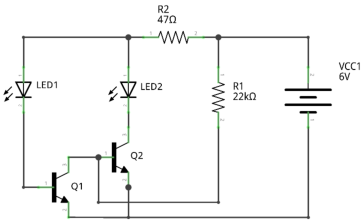
\includegraphics[scale=1.4]{Transistor/Schaltungen/NotBeleuchtung_Schaltplan.pdf}}
	\subfigure[Mögliche Breadboard-Ansicht]{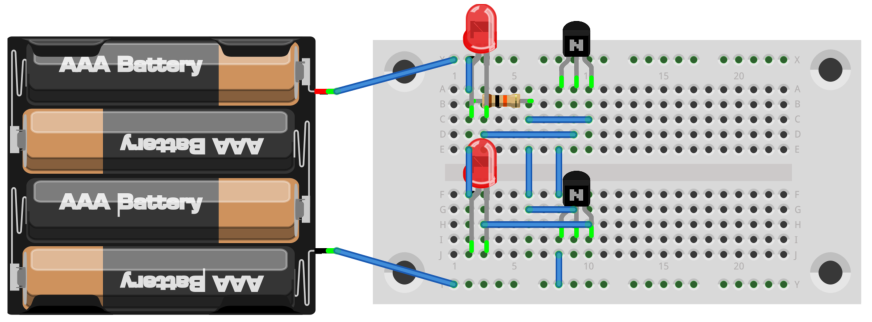
\includegraphics[scale=1]{Transistor/Schaltungen/NotBeleuchtung_Steckplatine.pdf}}
	\caption{Transistorschaltung 01 - Der Bipolar-Transistor als Schalter}
	\label{s01}
\end{figure}

%----------------------------------------------

\subsection[Der Bipolar-Transistor als Sensor]{Transistorschaltung 02 - Der Bipolar-Transistor als Sensor}

\begin{itemize}
\itemsep1pt\parskip0pt\parsep0pt
\item Bauen Sie folgende Transistor-Schaltung auf (Abbildung \ref{s02}). 
\item Legen Sie die Versorgungsspannung an die Schaltung an.
\item Berühren Sie die Basis des Transistors Q1 mit dem Finger. Was passiert und warum?
\end{itemize}

\begin{figure}[H]
	\centering
	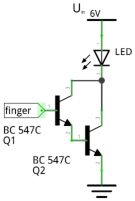
\includegraphics[scale=1.6]{Transistor/Schaltungen/NPN_Sensor.pdf}
	\caption{Transistorschaltung 02 - Der Bipolar-Transistor als Sensor}
	\label{s02}
\end{figure}

%----------------------------------------------

\subsection[Der Bipolar-Transistor als Verstärker]{Transistorschaltung 03 - Der Bipolar-Transistor als Verstärker}

\begin{itemize}
\itemsep1pt\parskip0pt\parsep0pt
\item Bauen Sie folgende Transistor-Schaltung auf (Abbildung \ref{s03}). 
\item Legen Sie die Versorgungsspannung an die Schaltung an.
\item Legen Sie ein Audiosignal an den Eingang der Schaltung an. Was passiert und warum?
\end{itemize}

\begin{figure}[H]
	\centering
	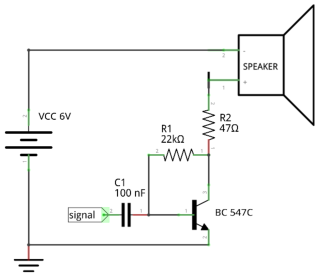
\includegraphics[scale=1.6]{Transistor/Schaltungen/NPN_Verstaerker.pdf}
	\caption{Transistorschaltung 03 - Der Bipolar-Transistor als Sensor}
	\label{s03}
\end{figure}

\chapter{Der Kurzwellendetektor}
 \begin{wrapfigure}[0]{r}[-1cm]{1cm}
   \vspace{-6cm}
   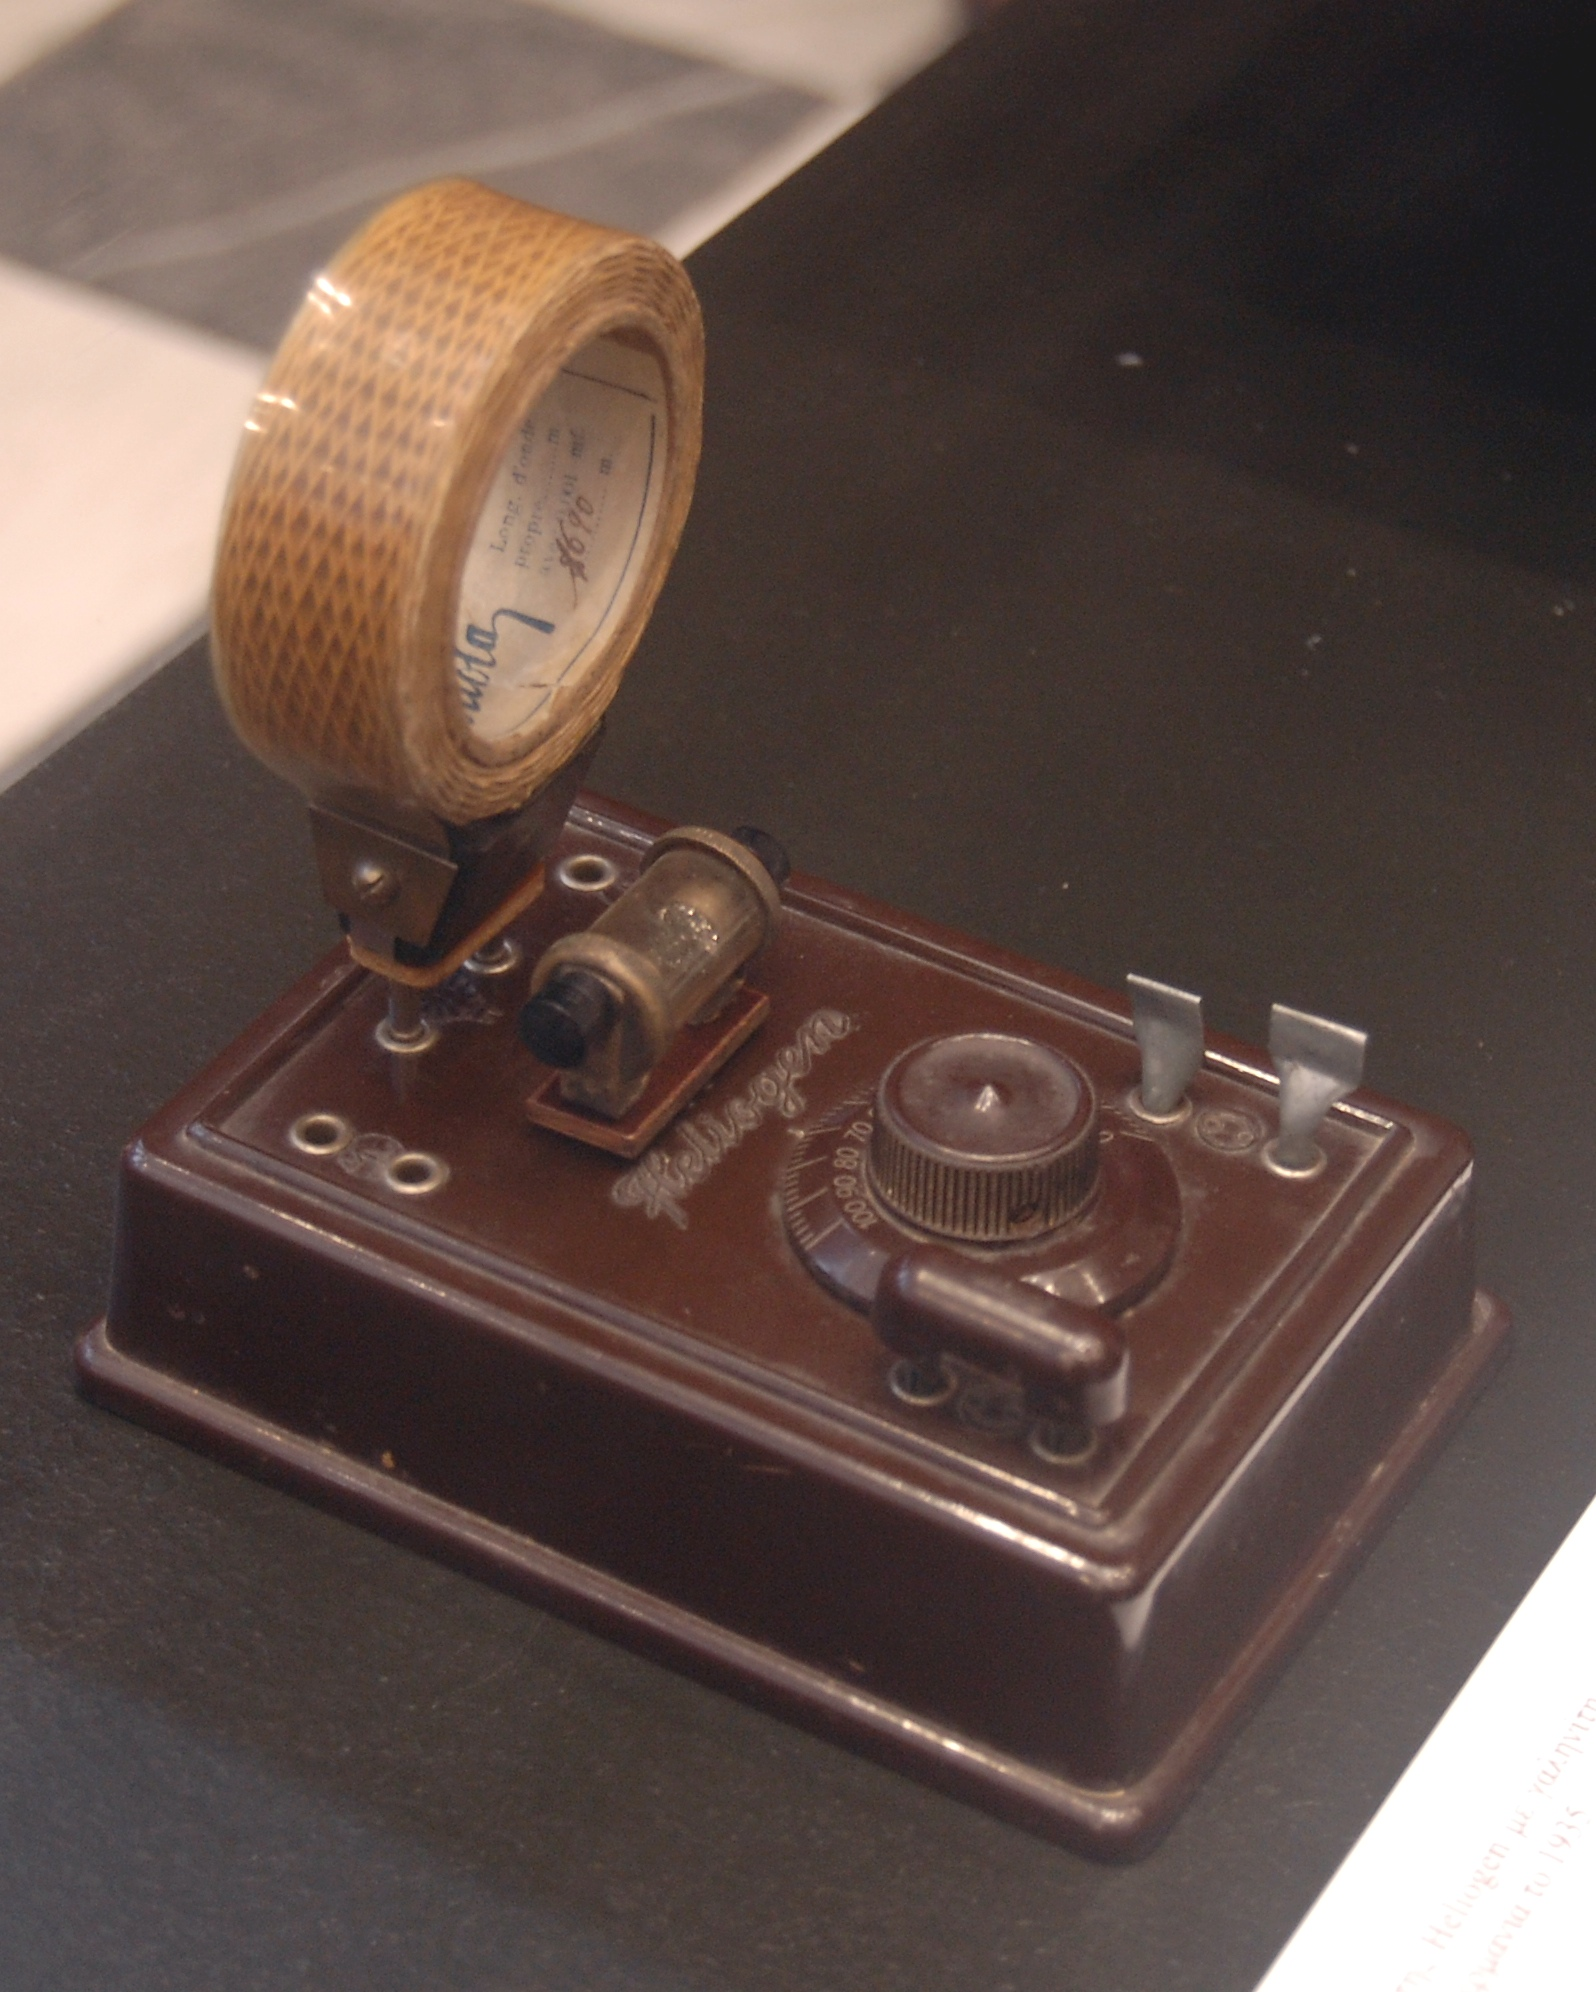
\includegraphics[scale=0.07]{Kurzwellendetektor/Bilder/Heliogen_medium_wave_galena_radio.JPG}
  \vspace{-6cm}
 \end{wrapfigure}

\section*{Praktische Anwendung}

\loesung{Mit den Lautsprechern funktioniert es ganz gut. Ggf. können sich die
SWL Kopfhörer mitbringen und diese mit einem Klinkenbuchsenadapter direkt
``anstöpseln.''

Mit der Spule um die $2.5 \mu H$ und dem DrehKo um die $200 pF$ befindet man
sich irgendwo im 40m-Band. Da Kurse meist Nachmittags/Abends stattfinden, bietet
sich dieses Band an. Für schnelle Erfolge kann man einen TRX mitnehmen und auf
dem Band in AM senden.

}

Radio- und Funk-Signale empfangen ohne die Verwendung einer Batterie oder einer
anderen Energiequelle? Eine einfache Schaltung ermöglicht das. Die folgende
Schaltung eines Detektorempfängers ist die einfachste aller Radioschaltungen. In
der Frühzeit der Radiotechnik war das Konzept eines Detektorempfänger durchaus
verbreitet, da es den Rundfunkempfang mit wenigen Bauteilen ermöglichst. Heute
ist es leider nich mehr ohne weiters möglich Radio-Sendungen mit dem der
Kurzwellendetektor zu empfangen, da der Großteil der Kurz- und
Mittelwellensender ihren Betrieb eingestellt haben. Nichts desto trotz ist er
ein guter Einstieg und ein technisches Abenteuer.

\begin{enumerate}
    %\itemsep1pt\parskip0pt\parsep0pt
  \item Berechnet die minimale und maximale Frequenz eines Schwingkreis mit
    eurer Spule (ggf. nochmal mit dem LC-Meter nachmessen) und einem
    Plattenpaket des DrehKos. Die minimal einstellbare Kapazität liegt bei ca.
    $5 pF$. Welche Afu-Bänder liegen in dem Bereich?  \loesung{Bei einer Spule
    um die $2.5 uH$ ist der Schwingkreis zwischen ca. 6 und 45 MHz tunebar.
    Bänder: Alle KW-Bänder ab 40m bis 10m.}
  \item Baue die Schaltung aus Abbildung \ref{kd} mit der bereits gebauten
    Spule und einem so genannten Langdraht als Antenne auf -- die länge der
    Antenne ist für den Empfang erstmal nicht so relevant. Bei dem
    eigentlichen "`Detektor"' handelt es sich um eine Germaniumdiode (z.B. AA
    143). Etwas weniger gut, aber weitaus preiswerter ist die Verwendung einer
    Schottky-Diode (z.B. BAT 43).  Was könnte die Diode tun und warum
    verwendet man keine Si-Dioden?
    \loesung{Dies ist ein Vorgriff auf die AM-Modulation. Die Diode
    demoduliert je nach Polung die obere oder untere Einhüllende.
    Germanium/Schottky-Dioden haben eine Schwellenspannung von ca. $0.3 V$,
    Silizium-Dioden arbeiten erst ab $0.6 V$ bis $0.7 V$.}
  \item Abgestimmt wird der Detektor mit dem DrehKo (gegen den Uhrzeigersinn
    gedreht wird die Kapazität größer). Mit diesem einfachen Aufbau können nur
    wirklich starke Sender empfangen werden -- wir simulieren das mit einem
    Funkgerät.  Mit etwas Glück kann aber auch ein echter Sender empfangen
    werden.
  \item Verwende den zuvor gebauten Audio-Verstärker, um empfangene Signale
    besser hörbar zu machen.
  \item Messt mit Hilfe des LC-Meters euren DrehKo aus und berechnet den
    Schwingkreis. In welchem Band werden die Signale der Antenne empfangen?
    \loesung{Die Spule hat um die $2.5 uH$ und der DrehKo max. $265 pF$ Die SWL
    sollen das schön per Hand rechnen. Zum Nachprüfen kann man z.B. dieses Tool
    verwenden: \url{http://wetec.vrok.de/rechner/cskreis.htm}}
\end{enumerate}

% TODO Kann man den Empfang mit einem anderen Spulenanzapf verbessern?

\begin{figure}[H]
    \centering
    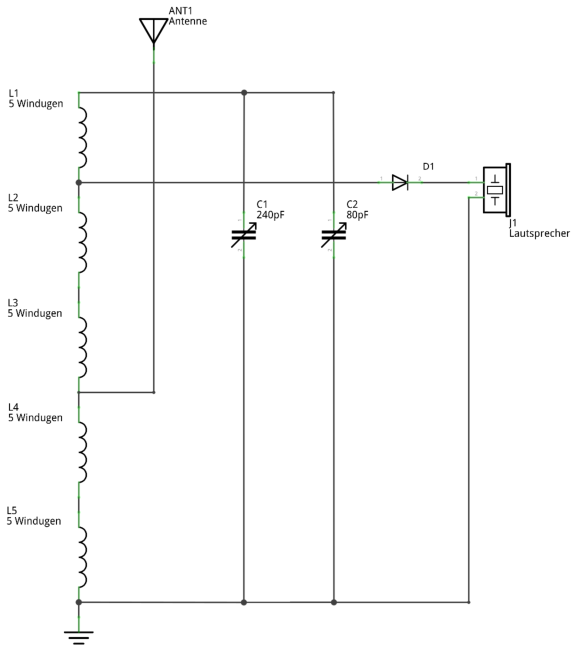
\includegraphics[scale=0.9]{Kurzwellendetektor/Bilder/Kurzwellendetektor_Schaltplan.pdf}
    \caption{Der Kurzwellendetektor}
    \label{kd}
\end{figure}


% Literaturverzeichnis
\bibliographystyle{natdin}
\addcontentsline{toc}{section}{Literaturverzeichnis}
\bibliography{Literaturverzeichnis}
% Abbildungsverzeichnis
\newpage
\addcontentsline{toc}{section}{Abbildungsverzeichnis}
\listoffigures	
%Anhang

\end{document}


